\chapter{Systemarkitektur}

\section{Hardware arkitektur}

Efterfølgende diagrammer viser hvordan hardware arkitekturen er opbygget.\footnote{For yderlige BBD/IBD se projektdokumentation afsnit System Artitektur.}

\begin{figure}[htbp] \centering
\section{Domænemodel}
{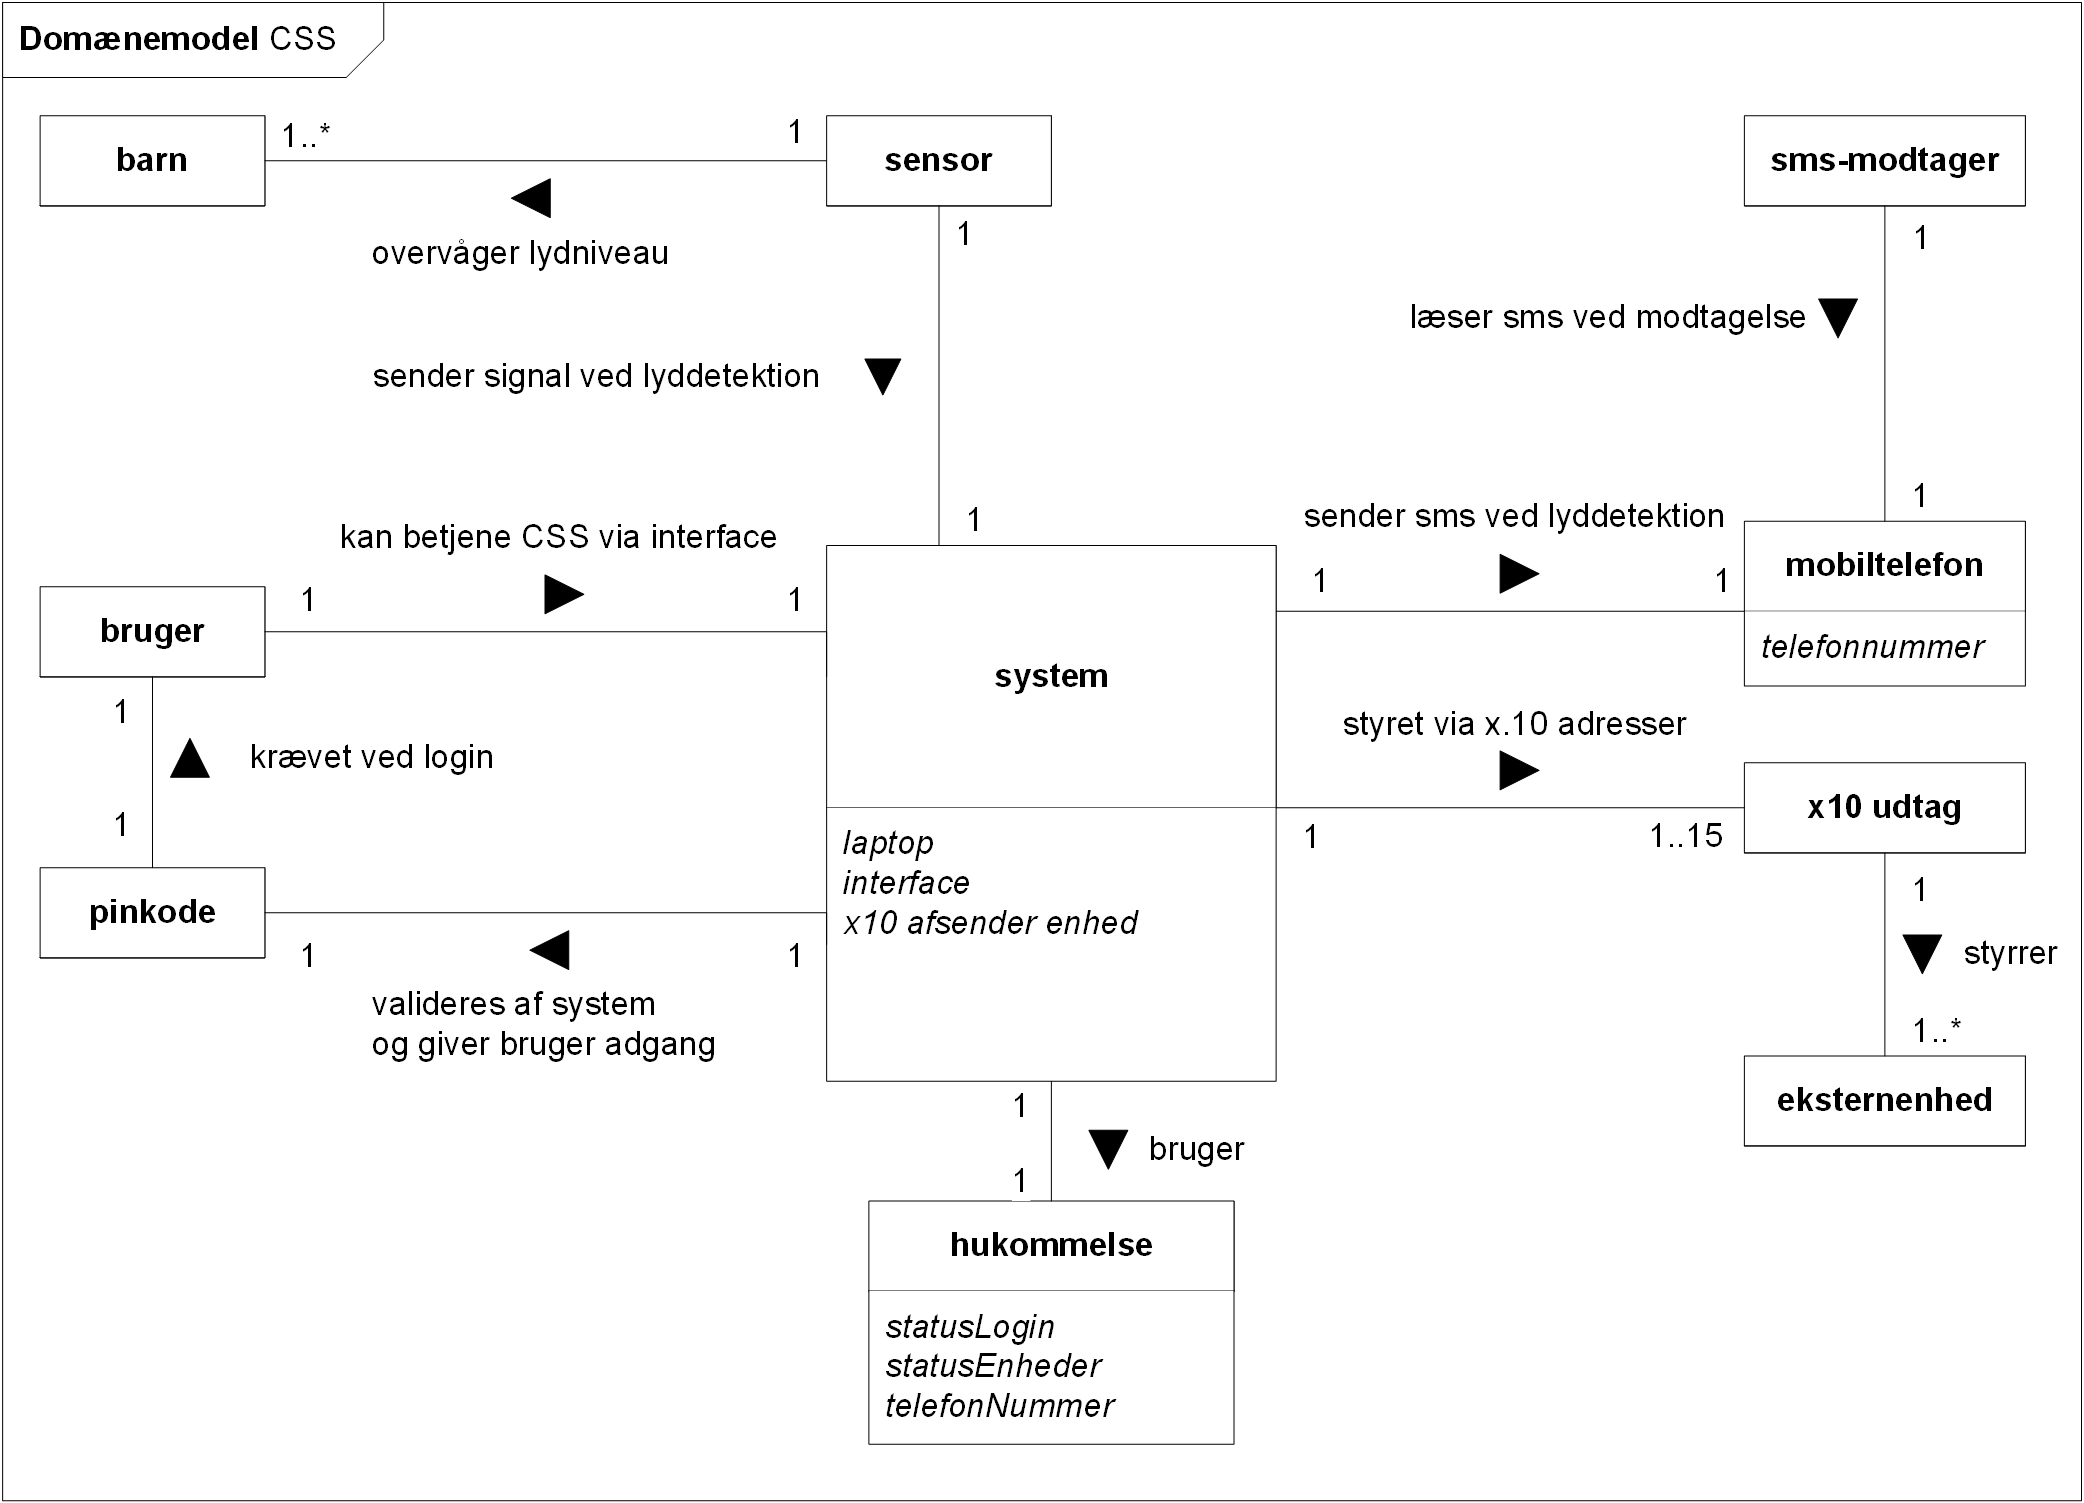
\includegraphics[width=\textwidth]{billeder/diagrammer/Domain_Model}}
\caption{Domænemodel}
\label{lab:domainmodel}
\end{figure}
Domænemodel er udarbejdet i samarbejde med kunden. Denne har til opgave at give et struktureret billede af systemets funktionalitet og sammenhæng. Domænemodellen gør ikke brug af fagudtryk, men pile og kortfattede samt præcise sætninger anvendes for at beskrive sammenhængen mellem blokkene. Dette er med til at opnå en højere forståelse, af systemet som helhed, for kunden.

\newpage

\begin{figure}[!htbp] \centering
\subsection{BDD Hardware}
{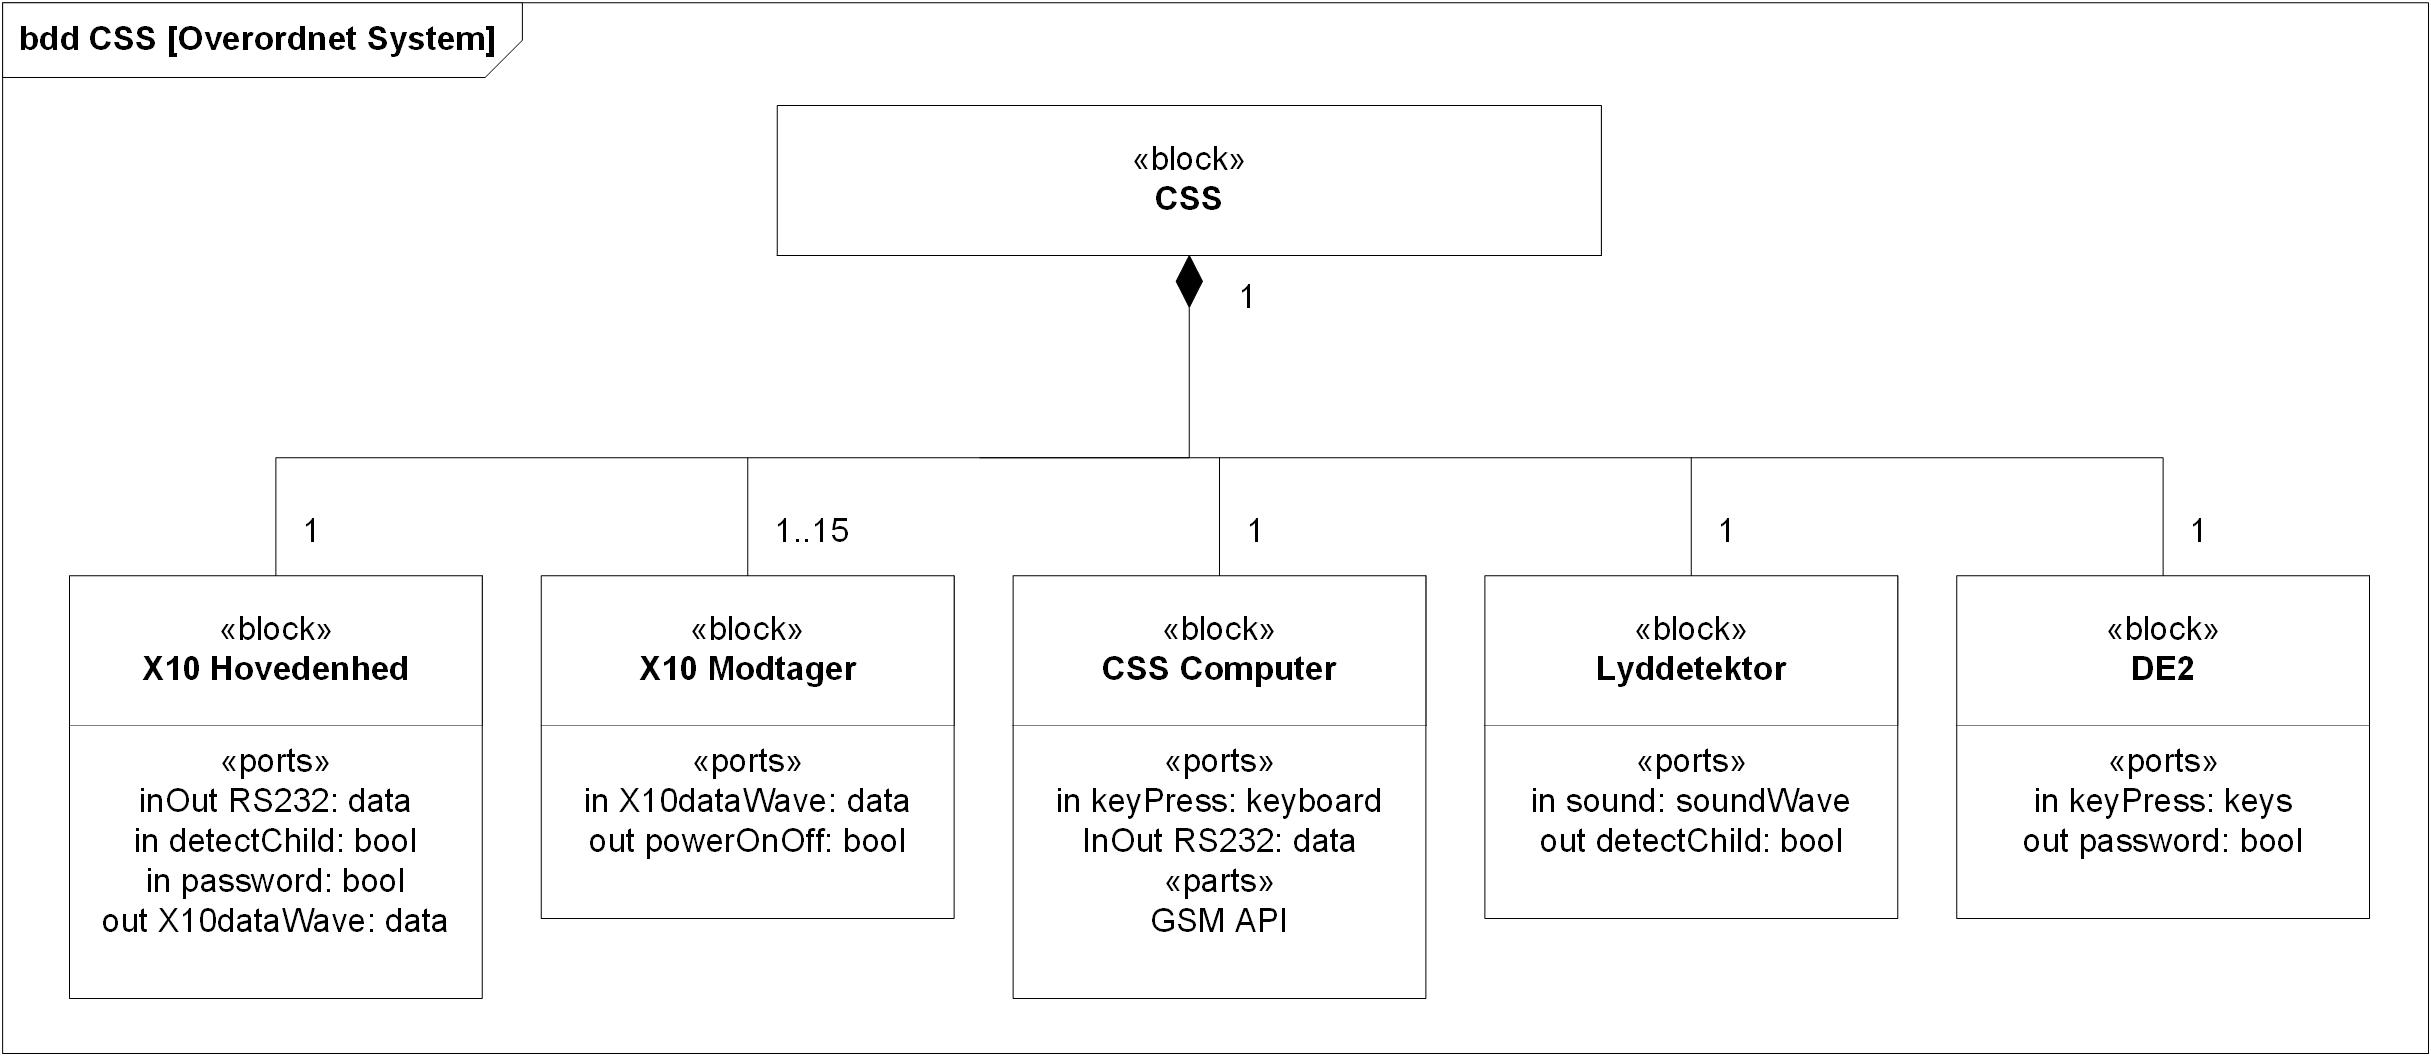
\includegraphics[width=0.9\textwidth]{billeder/diagrammer/BDD_Hardware}}
\caption{BDD Hardware}
\label{lab:bddhardware}
\raggedright
\end{figure}
BDD diagrammet giver et overblik over hvad det samlede system består af. Vi ser en port beskrivelse som viser hvilke signaler hver blok består af.


\begin{figure}[!htbp] \centering
\subsection{Plantegning over HW}
{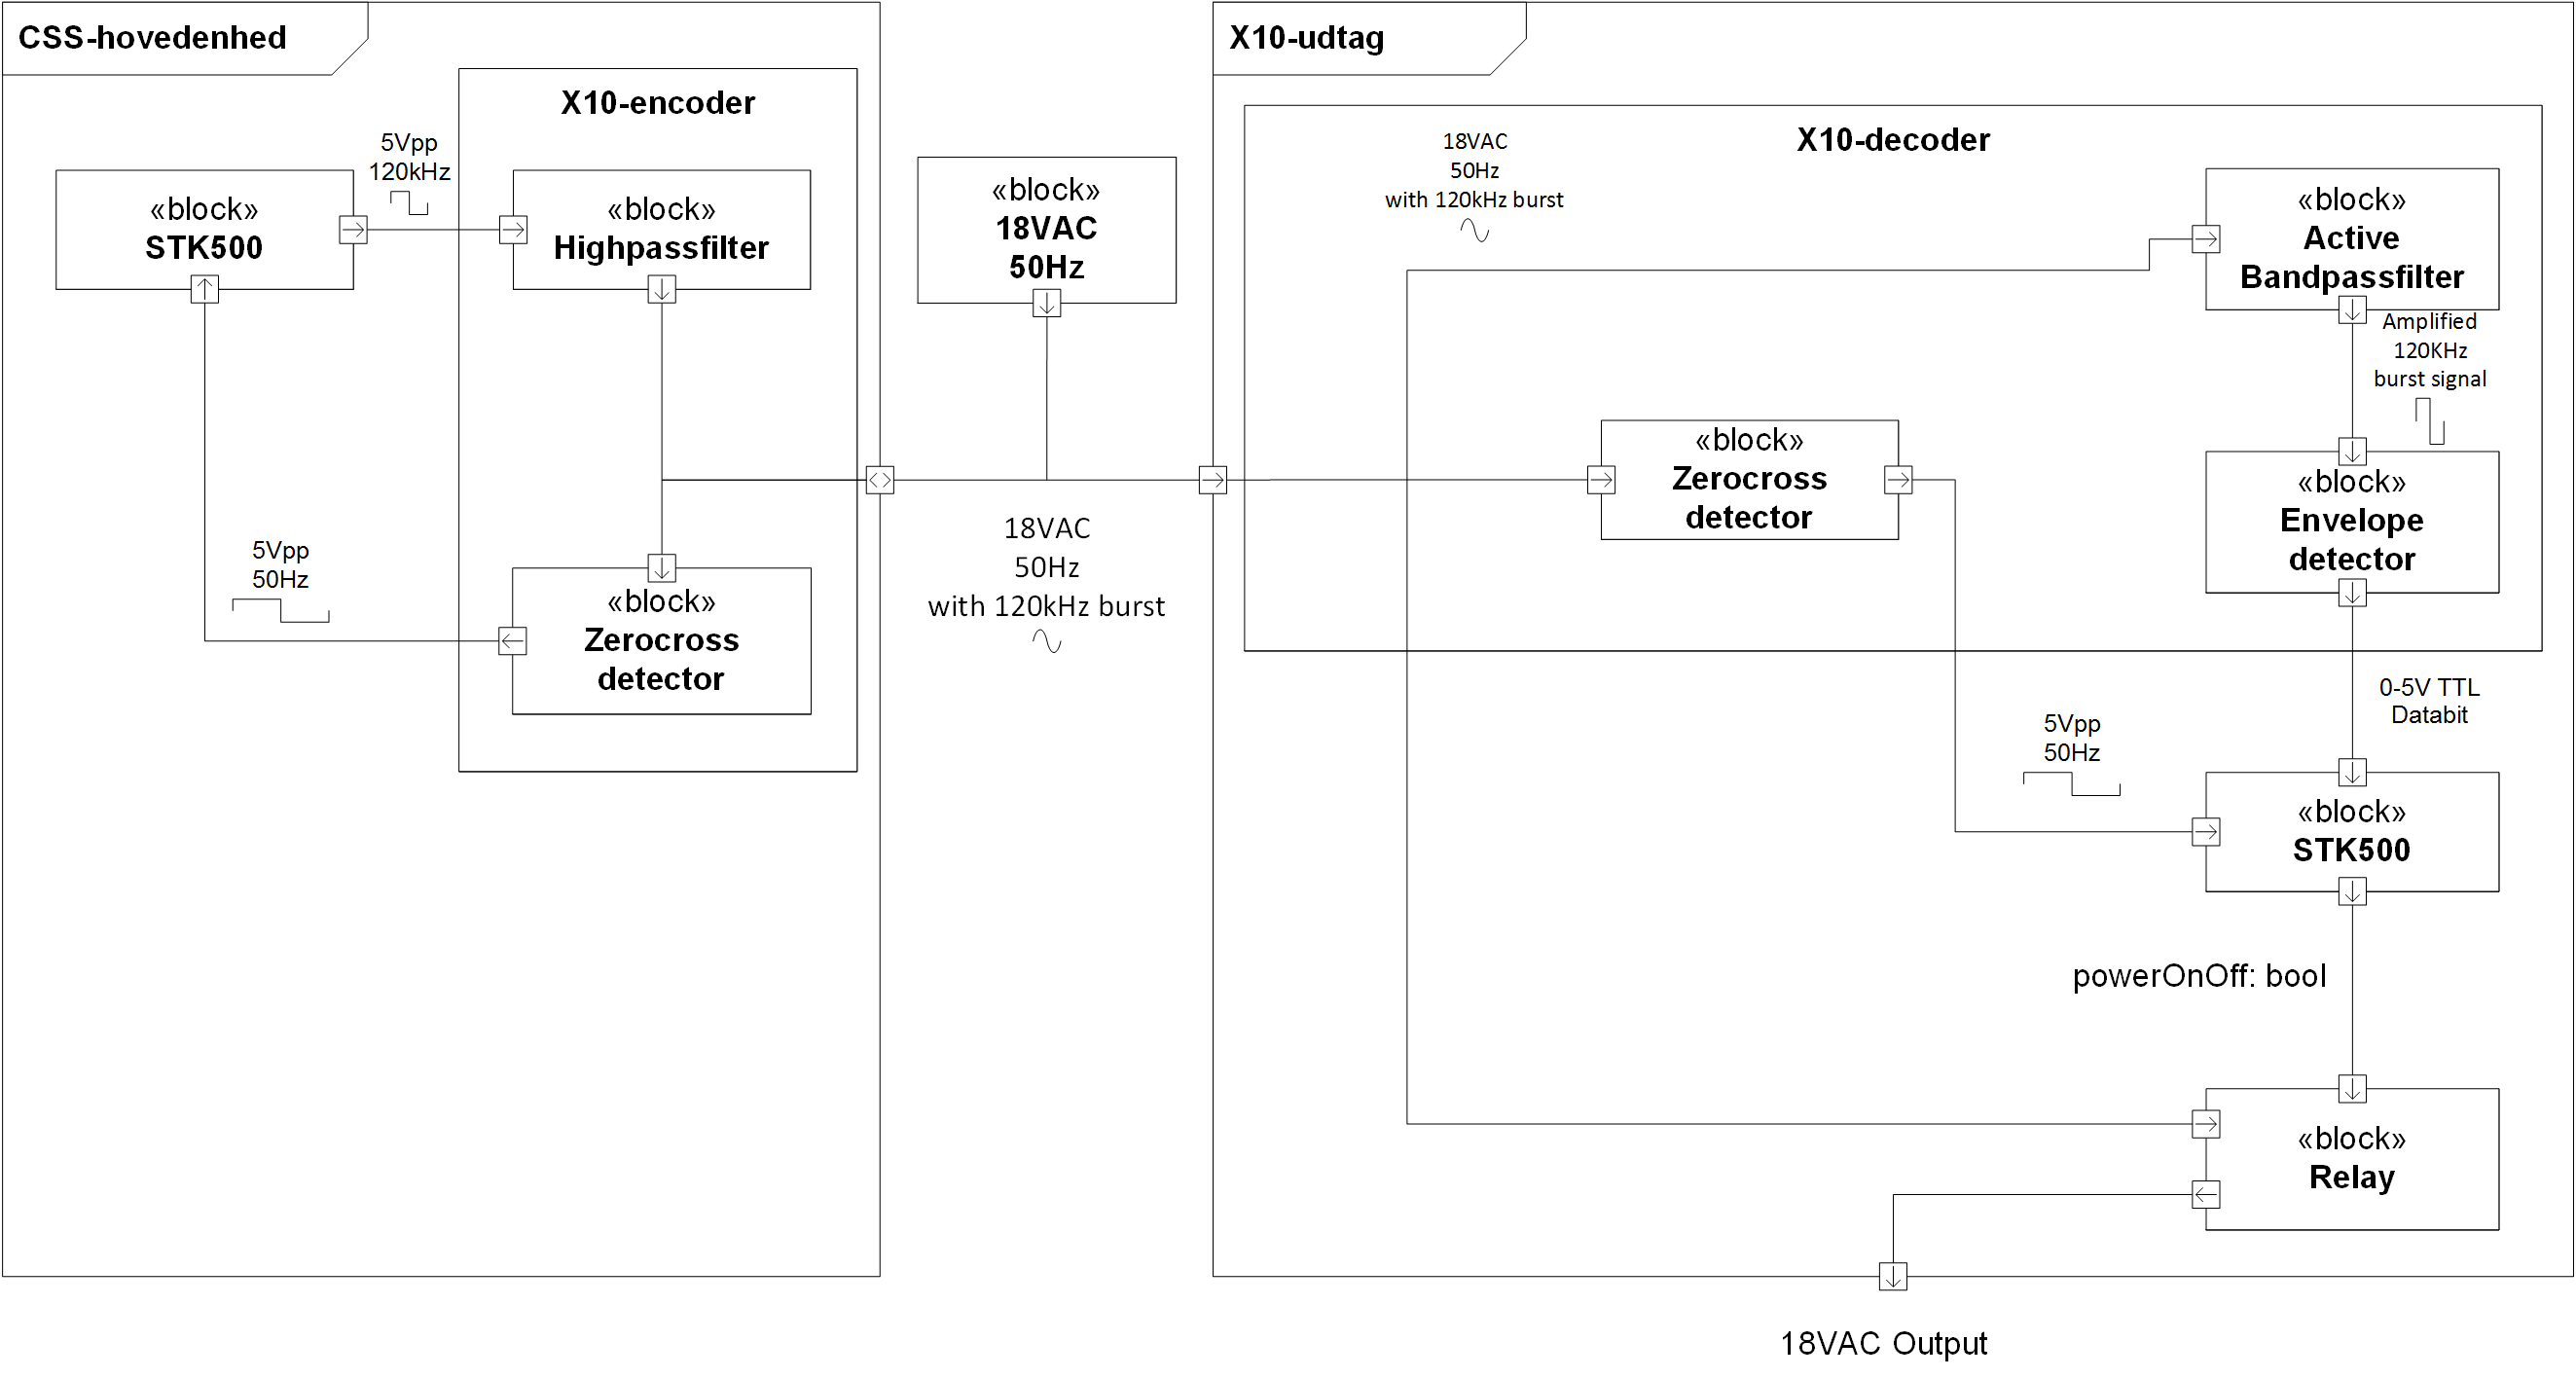
\includegraphics[width=0.9\textwidth]{billeder/diagrammer/Plantegning_over_HW}}
\caption{Plantegning over HW}
\label{lab:Plantegning over HW}
\raggedright
\end{figure}
Plantegningen over HW giver et overblik over hvordan CSS hovedenheden og X10-udtaget er forbundet, samt hvilken type signaler der bliver sendt imellem dem.

\clearpage

\section{Software arkitektur}
\subsection{PC}

\subsection{CSS hovedenhed}

\subsection{CSS udtag}